\documentclass[journal,12pt,twocolumn]{IEEEtran}

\usepackage{setspace}
\usepackage{gensymb}
\singlespacing
\usepackage[cmex10]{amsmath}

\usepackage{amsthm}

\usepackage{mathrsfs}
\usepackage{txfonts}
\usepackage{stfloats}
\usepackage{bm}
\usepackage{cite}
\usepackage{cases}
\usepackage{subfig}

\usepackage{longtable}
\usepackage{multirow}

\usepackage{enumitem}
\usepackage{mathtools}
\usepackage{steinmetz}
\usepackage{tikz}
\usepackage{circuitikz}
\usepackage{verbatim}
\usepackage{tfrupee}
\usepackage[breaklinks=true]{hyperref}
\usepackage{graphicx}
\usepackage{tkz-euclide}

\usetikzlibrary{calc,math}
\usepackage{listings}
    \usepackage{color}                                            %%
    \usepackage{array}                                            %%
    \usepackage{longtable}                                        %%
    \usepackage{calc}                                             %%
    \usepackage{multirow}                                         %%
    \usepackage{hhline}                                           %%
    \usepackage{ifthen}                                           %%
    \usepackage{lscape}     
\usepackage{multicol}
\usepackage{chngcntr}

\DeclareMathOperator*{\Res}{Res}

\renewcommand\thesection{\arabic{section}}
\renewcommand\thesubsection{\thesection.\arabic{subsection}}
\renewcommand\thesubsubsection{\thesubsection.\arabic{subsubsection}}

\renewcommand\thesectiondis{\arabic{section}}
\renewcommand\thesubsectiondis{\thesectiondis.\arabic{subsection}}
\renewcommand\thesubsubsectiondis{\thesubsectiondis.\arabic{subsubsection}}


\hyphenation{op-tical net-works semi-conduc-tor}
\def\inputGnumericTable{}                                 %%

\lstset{
%language=C,
frame=single, 
breaklines=true,
columns=fullflexible
}
\begin{document}

\newcommand{\BEQA}{\begin{eqnarray}}
\newcommand{\EEQA}{\end{eqnarray}}
\newcommand{\define}{\stackrel{\triangle}{=}}
\bibliographystyle{IEEEtran}
\raggedbottom
\setlength{\parindent}{0pt}
\providecommand{\mbf}{\mathbf}
\providecommand{\pr}[1]{\ensuremath{\Pr\left(#1\right)}}
\providecommand{\qfunc}[1]{\ensuremath{Q\left(#1\right)}}
\providecommand{\sbrak}[1]{\ensuremath{{}\left[#1\right]}}
\providecommand{\lsbrak}[1]{\ensuremath{{}\left[#1\right.}}
\providecommand{\rsbrak}[1]{\ensuremath{{}\left.#1\right]}}
\providecommand{\brak}[1]{\ensuremath{\left(#1\right)}}
\providecommand{\lbrak}[1]{\ensuremath{\left(#1\right.}}
\providecommand{\rbrak}[1]{\ensuremath{\left.#1\right)}}
\providecommand{\cbrak}[1]{\ensuremath{\left\{#1\right\}}}
\providecommand{\lcbrak}[1]{\ensuremath{\left\{#1\right.}}
\providecommand{\rcbrak}[1]{\ensuremath{\left.#1\right\}}}
\theoremstyle{remark}
\newtheorem{rem}{Remark}
\newcommand{\sgn}{\mathop{\mathrm{sgn}}}
\newcommand{\comb}[2]{{}^{#1}\mathrm{C}_{#2}}
\providecommand{\abs}[1]{\vert#1\vert}
\providecommand{\res}[1]{\Res\displaylimits_{#1}} 
\providecommand{\norm}[1]{\lVert#1\rVert}
%\providecommand{\norm}[1]{\lVert#1\rVert}
\providecommand{\mtx}[1]{\mathbf{#1}}
\providecommand{\mean}[1]{E[ #1 ]}
\providecommand{\fourier}{\overset{\mathcal{F}}{ \rightleftharpoons}}
%\providecommand{\hilbert}{\overset{\mathcal{H}}{ \rightleftharpoons}}
\providecommand{\system}{\overset{\mathcal{H}}{ \longleftrightarrow}}
	%\newcommand{\solution}[2]{\textbf{Solution:}{#1}}
\newcommand{\solution}{\noindent \textbf{Solution: }}
\newcommand{\cosec}{\,\text{cosec}\,}
\providecommand{\dec}[2]{\ensuremath{\overset{#1}{\underset{#2}{\gtrless}}}}

\newcommand{\myvec}[1]{\ensuremath{\begin{pmatrix}#1\end{pmatrix}}}
\newcommand{\mydet}[1]{\ensuremath{\begin{vmatrix}#1\end{vmatrix}}}
\numberwithin{equation}{subsection}
\makeatletter
\@addtoreset{figure}{problem}
\makeatother
\let\StandardTheFigure\thefigure
\let\vec\mathbf
\renewcommand{\thefigure}{\theproblem}
\def\putbox#1#2#3{\makebox[0in][l]{\makebox[#1][l]{}\raisebox{\baselineskip}[0in][0in]{\raisebox{#2}[0in][0in]{#3}}}}
     \def\rightbox#1{\makebox[0in][r]{#1}}
     \def\centbox#1{\makebox[0in]{#1}}
     \def\topbox#1{\raisebox{-\baselineskip}[0in][0in]{#1}}
     \def\midbox#1{\raisebox{-0.5\baselineskip}[0in][0in]{#1}}
\vspace{3cm}
\title{Assignment 2}
\author{Challa Akshay Santoshi-CS21BTECH11012}
\maketitle
\newpage
\bigskip
\renewcommand{\thefigure}{\theenumi}
\renewcommand{\thetable}{\theenumi}
\begin{center}
  \textbf{\underline{ICSE 12 2019}}\\
\end{center}
\begin{center}
  \textbf{Question: 20 (b)}  
\end{center}
Find the equation of the regression line of y on x, if the observations (x, y) are as follows:\\
(1, 4), (2, 8), (3, 2), (4, 12), (5, 10), (6, 14), (7, 16), (8, 6), (9, 18)\\
Also find the estimated value of y when x = 14.\\
\begin{center}
  \textbf{Solution:}  
\end{center}
Let the regression line of Y on X be given by
\begin{align}
    y = A + Bx
\end{align}
Here 'A' is the Y-intercept and 'B' is the slope of the line.\\
Using vectors, it can also be represented as:
\begin{align}
    \myvec{B & -1}\vec{X} = -A
\end{align}
From the definition of line regression, the value of 'B' can be found from a set of data using following relation:\\
\begin{align}
    B = \frac{\Sigma xy - \frac{\Sigma x \Sigma y}{n}}{\Sigma x^2 - \frac{(\Sigma x)^2}{n}}
\end{align}
So, equation (0.0.2) can be written as:\\
\begin{align}
    \myvec{\frac{\Sigma xy - \frac{\Sigma x \Sigma y}{n}}{\Sigma x^2 - \frac{(\Sigma x)^2}{n}} & -1}\vec{X} = -A
\end{align}
To find the value of 'A', we can substitute the point $ \myvec{\frac{\Sigma x}{n} \\ \frac{\Sigma y}{n}}  $ in the equation (0.0.3) and solve for it.\\
Solving for 'A' we can simplify it as:\\
\begin{align}
    \myvec{\frac{\Sigma xy - \frac{\Sigma x \Sigma y}{n}}{\Sigma x^2 - \frac{(\Sigma x)^2}{n}} & -1}\myvec{\frac{\Sigma x}{n} \\ \frac{\Sigma y}{n}} = -A
\end{align}
Substituting this value of '-A' back in equation (0.0.4), we get the regression line of y on x as\\
\begin{align}
    \myvec{\frac{\Sigma xy - \frac{\Sigma x \Sigma y}{n}}{\Sigma x^2 - \frac{(\Sigma x)^2}{n}} & -1}\vec{X} = \myvec{\frac{\Sigma xy - \frac{\Sigma x \Sigma y}{n}}{\Sigma x^2 - \frac{(\Sigma x)^2}{n}} & -1}\myvec{\frac{\Sigma x}{n} \\ \frac{\Sigma y}{n}}
\end{align}\\

From the data given in question,\\\
\begin{align}
  \Sigma x  &= 1 + 2 + 3 + 4 + 5 + 6 + 7 + 8 + 9\\
 \Sigma y  &= 4 + 8 + 2 + 12 + 10 + 14 + 16 + 6 + 18\\
 \Sigma xy &= 4 + 16 + 6 + 48 + 50 + 84 + 112 + 48 + 162\\
 \Sigma x^2 &= 1 + 4 + 9 + 16 + 25 + 36 + 49 + 64 + 81\\
\end{align}
From these above equations we get,\\
\begin{align}
  \Sigma x  &= 45\\
 \Sigma y  &= 90\\
 \Sigma xy &= 530\\
 \Sigma x^2 &= 285\\
 n &= 9
\end{align}
Substituting these values in equation (0.0.6) will give\\
\begin{align}
    \myvec{\frac{530 - \frac{45 \times 90}{9}}{285 - \frac{(45)^2}{9}} & -1}\vec{X} &= \myvec{\frac{530 - \frac{45 \times 90}{9}}{285 - \frac{(45)^2}{9}} & -1}\myvec{\frac{45}{9} \\ \frac{90}{9}}
\end{align}\\
Simplifying we get
\begin{align}
    \myvec{\frac{80}{60} & -1}\vec{X} = \myvec{\frac{80}{60} & -1}\myvec{5 \\ 10}
    \\
    \implies \myvec{\frac{4}{3} & -1}\vec{X} = \frac{-10}{3}
\end{align}\\
Equation (0.0.19) gives us the linear equation\\
\begin{align}
    \frac{4}{3} x - y &= \frac{-10}{3}
\end{align}\\
Simplifying we get,
\begin{align}
    4x - 3y + 10 = 0 
\end{align}
Equation (0.0.21) is the required equation of the regression line of y on x for the data given.\\\\
The second part of the question asks us to find the estimated value of y when x = 14.\\
Using equation (0.0.19), we can find y as follows:\\
\begin{align}
    \myvec{\frac{4}{3} & -1}\myvec{14 \\ y} = \frac{-10}{3}
\end{align}
\begin{align}
    \implies \frac{56}{3} - y &= \frac{-10}{3}
\end{align}    
\begin{align}
   \implies y = \frac{66}{3}
\end{align}
\begin{align}
    \implies y &= 22 
\end{align}
Therefore, the value of y is 22 when x is 14.\\\\
Figure given below represents the regression line.
\begin{figure}[ht]
    \centering
    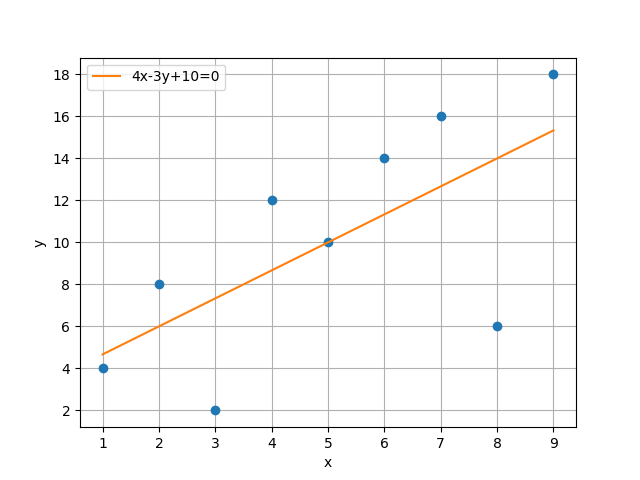
\includegraphics[width=\columnwidth]{Figure_1.png}
    \caption{Graph showing the Regression Line}
    \label{Figure_1}
\end{figure}
\end{document}